\documentclass[10pt]{article}
\usepackage[margin=0.8in]{geometry}
\usepackage{graphicx}
\usepackage{amssymb}
\usepackage[hidelinks]{hyperref}
\title{Certicom ECCp-131: scalar tensor reference}
\author{Implementation validation receipt}
\date{29 October 2026}
\begin{document}
\maketitle
\noindent\textbf{Status: implemented reference; challenge scalar unresolved.}
The prime-field counterpart requested as ``ECCp-130'' is officially named
ECCp-131 in \href{https://www.certicom.com/en/curves-list}{Certicom's curve list}.
The implementation uses its exact published parameters and cofactor one.
ECC2K-130 remains separately supported. Neither challenge is solved here.

\begin{center}
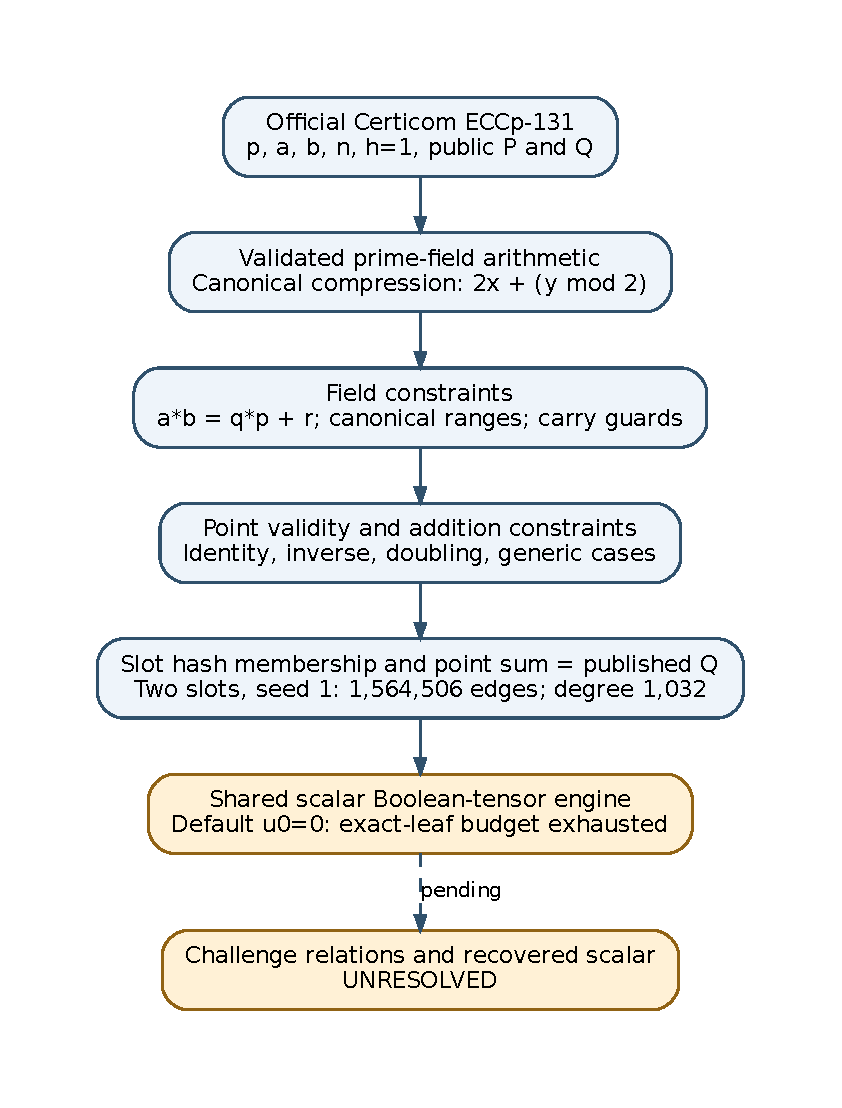
\includegraphics[height=4.9in,keepaspectratio]{pipeline.pdf}
\end{center}

\noindent The graph is a constraint pipeline, not an isogeny or a new curve
route. Solid arrows are implemented composition; the dashed arrow is an
unresolved challenge computation.

\newpage
\section*{Construction and checks}
The prime-field module implements short-Weierstrass arithmetic, Tonelli--Shanks
decompression and canonical encoding $2x+(y\bmod2)$. The coordinate module
reuses the integer Fourier multiplier and enforces bounded integer equations
$ab=qp+r$, canonical residues, addition/subtraction carries, exceptional point
addition cases, fixed-cofactor image witnesses, affine hash thresholds and
the target point sum. Test hints are absent from compiled tensor networks.

The combined suite passes 39 development tests with no skips: exhaustive
modular pairs over $\mathbb F_{17}$, all 361 pairs in an order-19 point group,
identity/inverse/zero-y/cofactor controls, invalid assignment rejection,
certificate corruption rejection and independent OpenSSL comparisons of 16
multiples of the published prime-field P/Q. A separate public indexed-tensor
fixture recovers scalar 7 and passes full relation-certificate replay.
Producer and certificate verifier share arithmetic; OpenSSL supplies an
independent arithmetic comparison, not a full proof of the tensor program.

The published target's two-slot, seed-1 network compiles to 1,564,506 edges,
654,523 variables and maximum degree 1,032. Compiled graph statistics agree
with construction statistics. The default policy selects $u_0=0$; exact
summation exceeds the 2,000,000-operation budget and exits 2 without a
challenge witness. Enumerating its factor bases also fails the 200,000-candidate
preflight. Neither failure proves nonexistence or a mathematical obstruction.

\section*{Scope and evidence}
These are retrospective development checks, not a benchmark or admitted
IC/rho comparison. Times in raw outputs are unisolated diagnostics.
No new mathematical theorem, novelty, Lean proof, asymptotic speedup, native
Rust integration or scientific cloud experiment is claimed. General
$\ell>1$, independent complete-encoding and complexity audits, native
integration and actual challenge relations/scalars remain open.

The companion directory retains commands, exit statuses, parameter/source
hashes, environment, test output, fixture certificate and failed challenge
receipts. The Markdown report (README.md) supplies exact reproduction commands,
source links and acceptance limits. Diagram source is pipeline.dot. Existing
native diagrams, reports and leaderboard rows are unchanged.

Sources: Certicom's official curve list; the pinned Bochum v0.2 paper; the
external October 25 contraction snapshots listed in reference/SOURCES.json;
the existing paired native reduction and canonical tensor-backend problem.
No formal verification of the external theorem follows from these checks.
\end{document}
